\documentclass[10pt]{article}
\usepackage[margin=0.56in]{geometry}
\usepackage{booktabs,enumitem,fancyhdr,graphicx,tabularx,titlesec}
\usepackage[table]{xcolor}
\usepackage[hidelinks]{hyperref}
\graphicspath{{docs/lessons/assets/}{../assets/}}
\hypersetup{pdftitle={ADK Lesson 051: Inert Parts Carousel},
 pdfauthor={Kevin Shanahan},
 pdfsubject={Transactional identity, confirmation, logical homing, inert position and gate intent, and fixed audit reconstruction},
 pdflang={en-US}}
\pagestyle{fancy}\fancyhf{}
\lhead{\textsc{ADK Lesson 051}}\rhead{Inert Parts Carousel}
\cfoot{\thepage}\setlength{\headheight}{14pt}
\setlength{\parindent}{0pt}\setlength{\parskip}{1.5pt}
\setlist{nosep,leftmargin=1.45em}
\titleformat{\section}{\Large\bfseries}{\thesection}{0.5em}{}
\titlespacing*{\section}{0pt}{7pt}{2pt}
\titlespacing*{\subsection}{0pt}{5pt}{2pt}
\newcommand{\lessonbox}[1]{\begin{center}\fbox{\parbox{0.92\linewidth}{#1}}\end{center}}
\newcommand{\blankline}{\rule{0.72in}{0.4pt}}

\begin{document}
\small
\begin{center}
 {\Huge\bfseries Inert Parts Carousel}\\[3pt]
 {\Large Admit, home, position, and audit one paper-bin request}\\[7pt]
 \fbox{\textbf{E0 SYNTHETIC REPLAY --- NO READER, STORAGE, MOTOR, SERVO, OR DISPENSING}}
\end{center}
\begin{tabularx}{\linewidth}{@{}>{\bfseries}l X >{\bfseries}l X@{}}
Lesson & 051 --- project & Time & 150--210 minutes\\
Prerequisites & Lessons 047, 049, 050 & Board & compile-only Mega replay\\
Evidence & result cells and fixture mirrors & Position & volatile logical coordinate only\\
\end{tabularx}

\lessonbox{\textbf{Project boundary.} \texttt{InertPartsCarousel} coordinates
copied synthetic identity, key, home, stop, and presentation evidence with
borrowed identity and homing policies, one privately owned logical sequencer,
semantic gate intent, and caller-owned audit bytes. It owns zero pins, timers,
interrupts, buses, endpoints, supplies, storage transports, or actuators.}

\section{Name the complete authorization invariant}
The project does not treat a local identifier as a credential or a person.
A known paper token selects a configured bin; an exact configured decimal
confirmation grants a short-lived project authorization. Even that
authorization cannot produce open-gate intent until every term below is true.

\begin{center}
% ADK visual: pencil
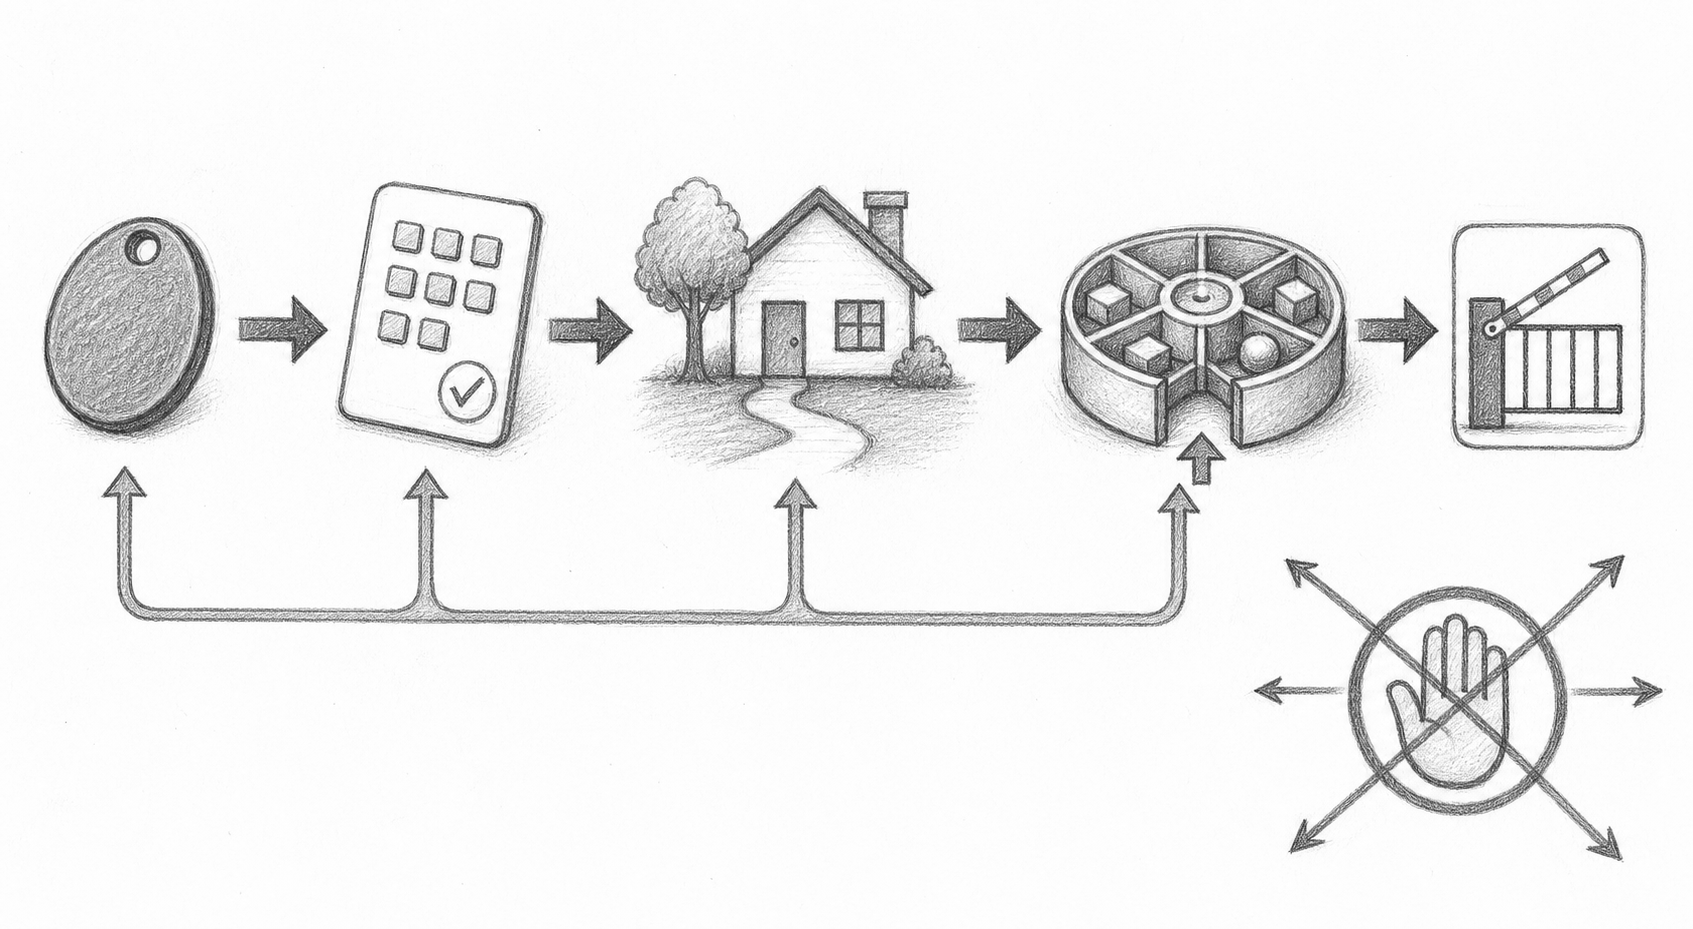
\includegraphics[width=0.96\linewidth,height=0.27\textheight,
 keepaspectratio]{051-invariant-path-pencil.png}

\small\textit{Alternative text: a pencil mnemonic links a round token, a
keypad with a check mark, a house, a divided carousel, and a barrier-gate
icon. A return line points back to the first four icons, while a crossed hand
with outward arrows appears below the carousel. The drawing contains no
labels, wiring, or powered hardware.}
\end{center}

\begin{tabularx}{\linewidth}{@{}l X@{}}
\toprule
Required term & Exact E0 meaning\\
\midrule
known identity & one binding in the committed caller-supplied image\\
matching confirmation & configured \(1\)--\(4\) digits, including leading zeros\\
durable admission & exact start record externally acknowledged from supplied bytes\\
successful home & fresh nonzero home epoch in this replay session\\
target reached & known logical coordinate equals the selected bin coordinate\\
healthy frame & current copied sources, valid time/skew, and inactive stop\\
\bottomrule
\end{tabularx}

The E0 result is a memory intent. It cannot authenticate an RFID card, prove
a keypad press, establish physical home, move a carousel, open a gate, retain
data through power loss, or dispense a part.

\section{Read one transactional frame}
Each accepted call admits one timestamped frame and commits at most one
bounded stage. Canonically absent identity and key payloads are fully zeroed;
their named synthetic source and status remain valid. A present key batch has
at most four qualified decimal digits and a zero tail.

\begin{enumerate}
 \item Independently validate stop before unrelated frame fields.
 \item Preflight identity, key, home, motion, presentation, and audit work.
 \item Reserve adjacent start and terminal audit slots before authorization.
 \item Export and acknowledge the exact start record before any motion intent.
 \item Home and position through at most one logical transition per frame.
 \item Publish bounded gate intent only after the full invariant holds.
 \item Restore closed and all-off intent before terminal reconciliation.
\end{enumerate}

Cancel dominates simultaneous confirm and digits. The collision records
\texttt{ConfirmationConflict} and grants no authority. Repeated source
sequences cannot add a digit. Authorization expires at its exact configured
boundary before a colliding confirmation.

\section{Coordinate two policies without partial motion}
\begin{center}
% ADK visual: pencil
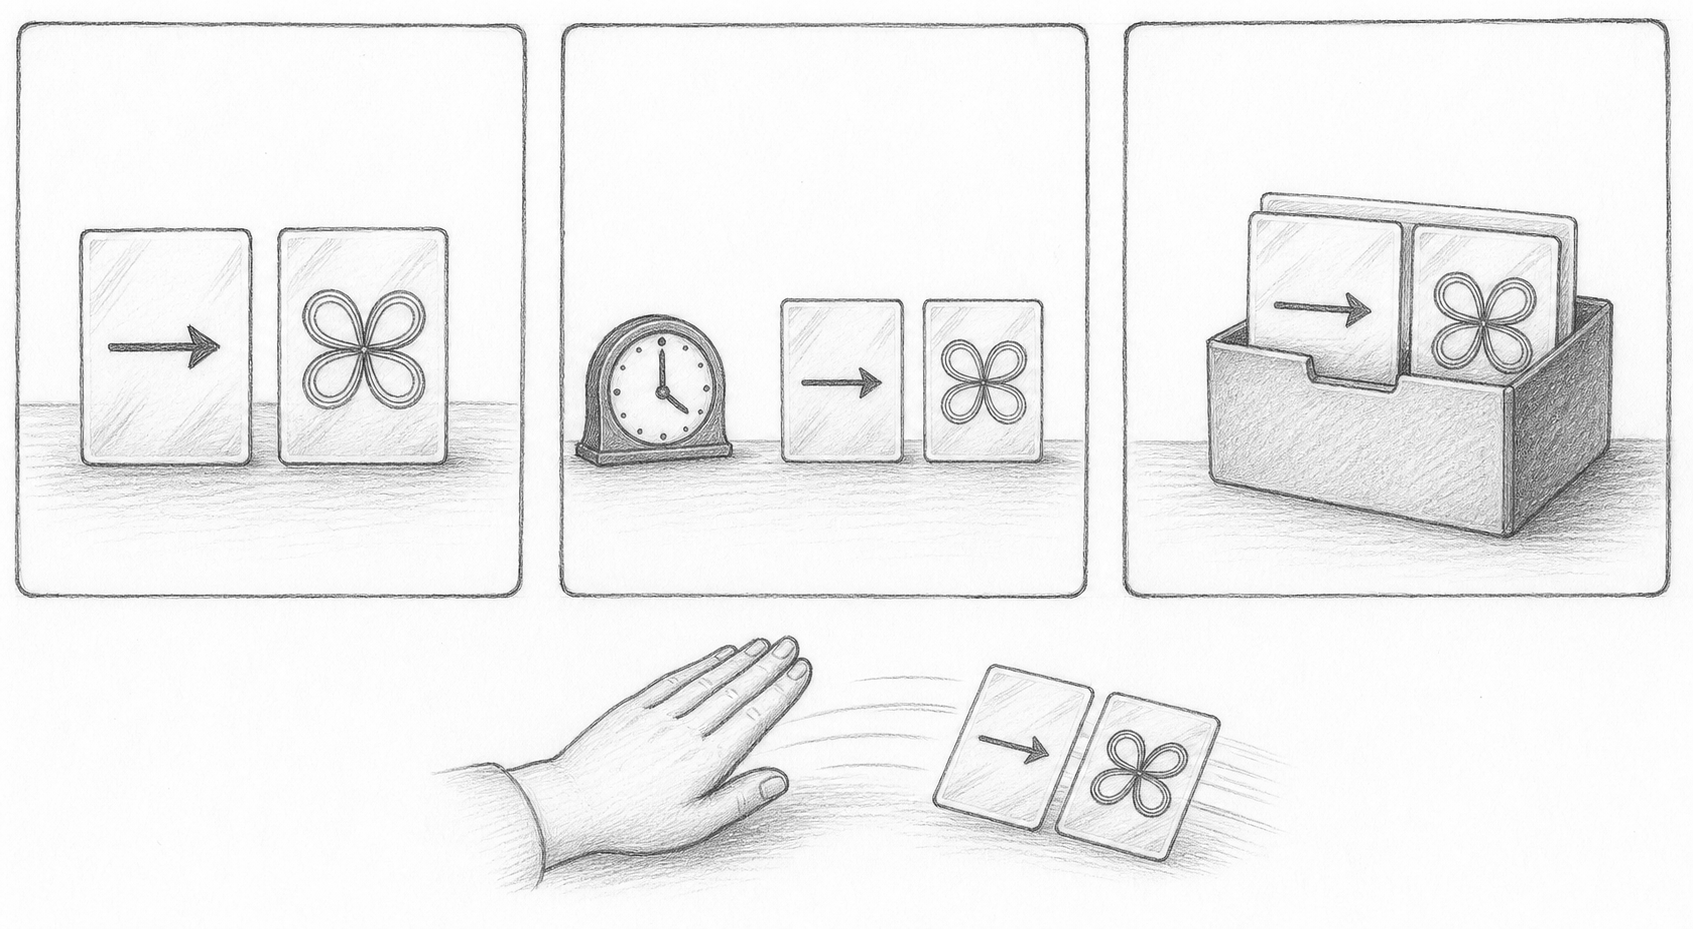
\includegraphics[width=0.95\linewidth,height=0.28\textheight,
 keepaspectratio]{051-joint-preview-pencil.png}

\small\textit{Alternative text: three pencil panels use paired cards marked
with an arrow and a four-loop symbol. The first places the cards side by
side, the second adds a clock, and the third places both cards in one box.
Below, a hand approaches a separate card pair. The drawing is a sequencing
mnemonic; it does not label previews, commits, coils, or hardware state.}
\end{center}

Lesson 050 supplies only a signed semantic step request. The project translates
that request to one exact Lesson 047 step, verifies both preview identities
and both \texttt{canCommit()} results, and commits each exactly once only after
no fallible work remains. Failure of either preview mutates neither policy.
Coil bits come only from the committed Lesson 047 snapshot.

The private sequencer uses native logical zero. Its checked signed bounds cover
every bin, zero, and the full Lesson 050 release/search excursion. There is no
offset, rebasing, inferred shaft coordinate, or persisted physical position.

\subsection*{Treat qualified home as a synchronization boundary}
On a new qualified home edge, the project derives but does not commit the
Lesson 050 preview. It directly stops the private sequencer only if live,
resets it unconditionally, and verifies logical zero, inactive phase, and
zero coil intent. Only then may Lesson 050 publish its new home epoch.
A stale preview cannot survive the reset generation change.

If direct stop or the zero/inactive/off check fails, the project stays all
off, latches \texttt{PositionFault}, leaves position unknown, and publishes no
home epoch. A simultaneous independent stop takes the stop path only.

\section{Let valid stop bypass unrelated faults}
A structurally valid, qualified active stop is the deliberate safety
exception. It is admitted before malformed identity, key, home, presentation,
or audit fields can delay it.

\begin{tabularx}{\linewidth}{@{}l X X@{}}
\toprule
Private sequencer & Stop action & Required result\\
\midrule
live or coils nonzero & direct \texttt{stop(now)} & coils zero, gate closed\\
idle and coils zero & do not mutate sequencer & home policy accepts stop\\
direct stop fails & all-off reset fallback & fault latched, no ordinary work\\
\bottomrule
\end{tabularx}

Stop cancels new authority and publishes closed/off intent. It never erases or
downgrades an already latched fault. A malformed stop cannot use this exception
and causes complete-frame rejection. Software stop intent is not an emergency
stop, a stationary mechanism, or independently removed actuator power.

\section{Open a semantic gate for bounded time}
\texttt{CarouselGateIntent::Open} is a semantic result with an explicit
expiry, not a servo pulse or physical gate state. At expiry the project first
restores \texttt{Closed} and zero coil intent, then advances toward completion
and terminal audit. No fault retries automatically.

\lessonbox{\textbf{No automatic dispensing.} A token, confirmation code,
logical home, or audit record never authorizes hazardous, valuable,
access-controlled, unattended, launcher, or safety-device operation.}

\newpage
\section{Reserve audit pairs before work begins}
Each operation owns two adjacent 40-byte canonical records: one acknowledged
authorization start and one terminal result. One remaining slot is
\texttt{AuditFull}; the project never leaves a start in the final slot.

\begin{center}
% ADK visual: pencil
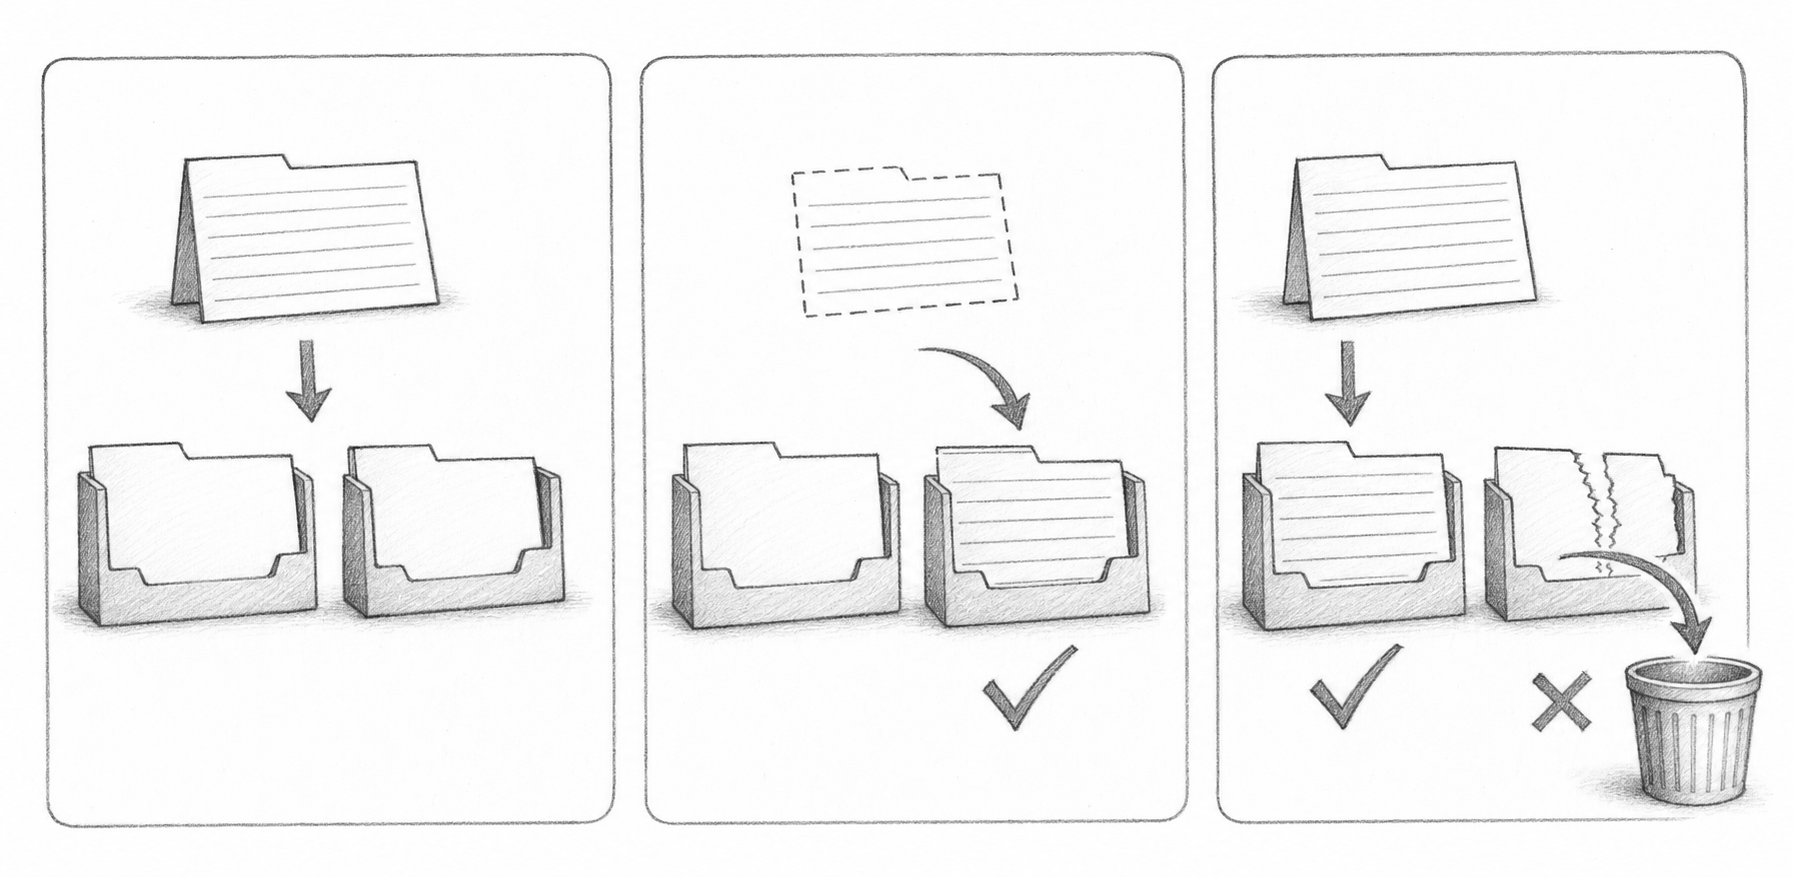
\includegraphics[width=0.95\linewidth,height=0.27\textheight,
 keepaspectratio]{051-audit-pairs-pencil.png}

\small\textit{Alternative text: three pencil panels show a lined card above
two adjacent file holders. The middle panel moves a dashed-outline card into
the right holder and adds a check mark. The final panel keeps the left card,
shows a torn card over the right holder, and points the torn pieces toward a
wastebasket beside a cross mark. The drawing does not number slots or encode
record contents.}
\end{center}

\begin{tabularx}{\linewidth}{@{}l r X@{}}
\toprule
Bytes & Offset & Canonical content\\
\midrule
4 & 0 & magic, schema version, encoded length\\
16 & 4 & project, operation, authorization, sequence, occurrence time\\
4 & 20 & kind, phase, bin, typed audit status\\
12 & 24 & identity digest/revision/image generation, home epoch\\
4 & 36 & two reserved zero bytes and CRC-16/CCITT-FALSE\\
\bottomrule
\end{tabularx}

The semantic C++ record is never persisted by its padded \texttt{sizeof}.
The codec writes unsigned little-endian fields, zero reserved bytes, and a
checksum over bytes \(0\)--\(37\). Valid capacities are exactly 2, 4, 6, or 8
records, with a 40-byte stride and a separate exact 40-byte candidate buffer.

\section{Acknowledge exact external evidence}
\texttt{previewAuditWrite()} and \texttt{previewAuditExport()} expose one
retryable candidate. An external coordinator may write, synchronize, reread,
and validate that candidate. \texttt{acknowledgeAuditWrite()} accepts only
matching owner, generation, operation, slot, view metadata, checksum, bytes,
synchronization, reread validation, and successful status.

A failed or indeterminate acknowledgement retains the candidate and blocks
replacement, reset, and new input work until reconciliation. An exact repeated
acknowledgement is idempotent; a changed repeat is an audit fault. These rules
prove deterministic supplied-image semantics, not atomic media writes,
retention, wear, or power-loss survival.

\section{Reconstruct without inventing history}
Recovery scans no more than eight slots and accepts only one canonical prefix.
A start with an erased reserved terminal becomes inhibited recovery work for
that same slot, operation, authorization, and identity binding. Recovery may
write only \texttt{Recovered\-Interrupted}; it cannot invent a new operation ID,
authorization epoch, home epoch, bin, or physical position.

Reject unsupported schema, wrong project identity, corrupt checksum,
noncanonical tail, terminal without start, mismatched pair fields, duplicate
terminal, invalid sequence delta, a start in the final slot, or a non-erased
mismatching reserved terminal. Restart begins gate closed, motion off, and
position unknown even when every audit byte is valid.

\newpage
\section{Run the deterministic E0 workbook}
\begin{enumerate}
 \item Start from two canonical identity images, empty audit bytes, unknown
       position, closed gate, and zero coil intent.
 \item Present one known copied token. Predict its exact bin, binding revision,
       and identity-image generation; then try unknown and repeated tokens.
 \item Enter the exact configured code, including a leading-zero case. Collide
       cancel with confirm and verify conflict without authorization.
 \item Export the start audit. Try foreign, changed, failed, and exact repeated
       acknowledgements before accepting the byte-identical record.
 \item Replay release-first homing. At the qualified home edge, predict private
       sequencer stop/reset, logical zero, all-off intent, then a new home epoch.
 \item Advance to the selected bin one due logical step per frame. Verify the
       coil mirror and that no gate-open intent precedes the complete invariant.
 \item Observe bounded semantic open intent, exact expiry, closed/off intent,
       and the matching terminal audit candidate.
 \item Collide valid stop with identity, confirmation, home, due step, arrival,
       gate expiry, audit-full, and presentation faults. Verify stop precedence.
 \item Restart with a start-only prefix. Predict inhibited, unknown-position
       recovery into only the reserved terminal slot.
 \item Inject corrupt pair fields, checksum, sequence ambiguity, full capacity,
       source fault, excessive skew, future time, rollover, shutdown, and a
       second byte-identical instance.
\end{enumerate}

\subsection*{E0 intent result cells}
\begin{tabularx}{\linewidth}{@{}X X X X X X@{}}
\toprule
frame & phase & bin & known? & logical position & home epoch\\
\midrule
\rule{0pt}{16pt}\blankline & \blankline & \blankline & \blankline & \blankline & \blankline\\[9pt]
\blankline & \blankline & \blankline & \blankline & \blankline & \blankline\\[9pt]
\blankline & \blankline & \blankline & \blankline & \blankline & \blankline\\
\bottomrule
\end{tabularx}

\begin{tabularx}{\linewidth}{@{}X X X X X X@{}}
\toprule
operation & authorized? & coil bits & gate intent & audit pending & fault\\
\midrule
\rule{0pt}{16pt}\blankline & \blankline & \blankline & \blankline & \blankline & \blankline\\[9pt]
\blankline & \blankline & \blankline & \blankline & \blankline & \blankline\\[9pt]
\blankline & \blankline & \blankline & \blankline & \blankline & \blankline\\
\bottomrule
\end{tabularx}

\section{Diagnose by precedence, not symptoms}
\begin{tabularx}{\linewidth}{@{}l X X@{}}
\toprule
Observed memory result & First question & Interpretation boundary\\
\midrule
\texttt{AuditFull} & are two adjacent slots free? & no partial authorization\\
\texttt{PositionFault} & did stop/reset/zero-off pass? & no physical diagnosis\\
\texttt{ConfirmationConflict} & cancel, confirm, overflow, repeat? & no credential claim\\
\texttt{AuditIndeterminate} & do reread bytes identify the candidate? & no durability claim\\
\texttt{PresentationFault} & did primary phase remain intact? & display is not authority\\
\bottomrule
\end{tabularx}

\newpage
\section{Interpret only what E0 observes}
\textbf{Acquisition prediction.} Canonical caller-owned buffers, valid child
configuration, and current copied sources allow initialization and replay
admission without claiming a hardware resource.

\textbf{Acquisition observation.} Host tests inspect lifecycle status,
typed dispositions, audit candidates, exact byte views, operation identity,
and complete snapshots in memory.

\textbf{Acquisition interpretation.} Success proves bounded policy
composition over copied data. It does not prove an RFID reader, keypad, home
sensor, display, storage medium, driver, motor, servo, or board was acquired.

\textbf{Safe-state prediction.} Construction, initialization, valid stop,
fault, interrupted recovery, shutdown, and restart publish closed gate and
zero coil intent; uncertain displacement leaves logical position unknown.

\textbf{Safe-state observation.} Inspect result cells, the private sequencer
mirror, terminal attribution, and supplied audit bytes.

\textbf{Safe-state interpretation.} All-off memory intent proves software
precedence only. It does not prove high impedance, de-energized windings,
stationary hardware, a closed gate, or removed actuator power.

\section{Keep the maximum fixture inside its gates}
The complete eight-binding/eight-bin fixture includes two 160-byte identity
images, one 160-byte identity candidate, at most eight 40-byte audit slots,
one 40-byte audit candidate, borrowed Lessons 049/050 objects, the private
Lesson 047 child, replay cells, and the coordinator.

Reusable children must remain at or below 128 bytes. The project coordinator
measures 380 bytes against its reviewed 320-byte target and 384-byte hard
ceiling. The Mega sketch measures 26,014 bytes flash and 1,933 bytes static
SRAM against ceilings of 28,672 and 2,048 bytes. The conservative live
stack/ISR path is 742 bytes and the reviewed reserve is 768 bytes, leaving
5,491 bytes after globals and that rounded reserve. Exceeding a gate stops for
design review; storage does not move to the heap.

\lessonbox{\textbf{Compile-only means compile-only.} A successful Mega build
proves that the public API and inert fixture fit the toolchain and recorded
budgets. It does not execute a result cell or qualify a powered circuit.}

\section{Leave E1 input and storage acceptance blank}
\lessonbox{\textbf{E1 remains open.} E1 may qualify exact low-energy input,
presentation, and nonvolatile-storage adapters while actuator power remains
absent. Supplied byte-image replay is not media durability evidence.}

\begin{tabularx}{\linewidth}{@{}>{\bfseries}l X@{}}
Exact RFID/keypad/home/stop specimens & \rule{0pt}{16pt}\hrulefill\\[9pt]
Primary datasheets and revision markings & \hrulefill\\[9pt]
Logic/supply levels, polarity, buses, and pin map & \hrulefill\\[9pt]
Exact display, LED, and resistor observation path & \hrulefill\\[9pt]
Exact nonvolatile medium and storage adapter & \hrulefill\\[9pt]
Write, sync, reread, rollback, and fault evidence & \hrulefill\\[9pt]
Resource acquisition evidence & \hrulefill\\[9pt]
Electrical safe-state evidence & \hrulefill\\[9pt]
Reviewer, date, acceptance record & \hrulefill\\
\end{tabularx}

\newpage
\section{Leave E2 powered carousel acceptance blank}
\lessonbox{\textbf{E2 remains open.} Do not add actuator wiring or power until
the exact restrained mechanism, motor/driver, servo, supplies, protection,
stop, and independent actuator-power removal are reviewed together.}

\begin{tabularx}{\linewidth}{@{}>{\bfseries}l X@{}}
Exact motor, winding, driver, and clamp topology & \rule{0pt}{16pt}\hrulefill\\[9pt]
Exact servo, gate geometry, and travel envelope & \hrulefill\\[9pt]
Electrically authoritative formal schematic & \hrulefill\\[9pt]
Separate current-limited actuator supply/common & \hrulefill\\[9pt]
Measured stepper, servo-stall, aggregate current & \hrulefill\\[9pt]
Thermal limits and de-energized hold behavior & \hrulefill\\[9pt]
Stable restraint, pinch guarding, lightweight load & \hrulefill\\[9pt]
Measured home, position, gate, stall, and collision & \hrulefill\\[9pt]
Independent stop and actuator-power removal & \hrulefill\\[9pt]
Named-person physical acceptance result & \hrulefill\\[9pt]
Reviewer, date, acceptance record & \hrulefill\\
\end{tabularx}

Future E2 work is limited to a stable, restrained, lightweight tabletop
demonstrator. It excludes loose or high-inertia loads, lifting, sharp
features, stored energy, vehicle or door-lock roles, unattended dispensing,
launcher control, and any safety function. Indicator light alone cannot prove
home, position, gate closure, de-energization, or independent power removal.

\section{Software evidence and further work}
Deterministic tests cover every bin and confirmation shape, full authorization
invariant, both homing directions, joint preview, live/idle/failing stop,
home synchronization, exact audit encoding and recovery, capacity edges,
collision precedence, shutdown, restart, maximum composition, and two-instance
fieldwise replay.

\begin{itemize}
 \item \href{https://github.com/spincyc/adk/blob/main/examples/Lesson051InertPartsCarousel/Lesson051InertPartsCarousel.ino}
       {Canonical compile-only Lesson 051 sketch}.
 \item \href{https://github.com/spincyc/adk/blob/main/tests/test_inert_parts_carousel.cpp}
       {Deterministic project tests}.
 \item \href{https://github.com/spincyc/adk/blob/main/src/inert_parts_carousel.h}
       {Inert-parts-carousel interface}.
 \item \href{https://github.com/spincyc/adk/blob/main/docs/design/LESSONS_049_051_PARTS_CAROUSEL_PLAN.md}
       {Lessons 049--051 design record}.
 \item \href{https://github.com/spincyc/adk/blob/main/docs/TESTING.md}
       {Deterministic testing contract}.
 \item \href{https://github.com/spincyc/adk/blob/main/docs/SAFETY_MODEL.md}
       {Safety model}.
\end{itemize}

This untagged print edition has a searchable HTML alternative.
It makes no PDF/UA, powered-input, storage-durability, motion, gate, dispensing,
or physical-position claim.
\end{document}
